%%%%%%%%%%%%%%%%%%%%%%%%%%%%%%%%%%%
%This is the LaTeX ARTICLE template for RSC journals
%Copyright The Royal Society of Chemistry 2016
%%%%%%%%%%%%%%%%%%%%%%%%%%%%%%%%%%%

\documentclass[twoside,twocolumn,9pt]{article}
\usepackage{tgheros}
\usepackage[utf8]{inputenc}
\renewcommand{\familydefault}{\sfdefault}

\usepackage{extsizes}
\usepackage[super,sort&compress,comma]{natbib} 
\usepackage[version=3]{mhchem}
\usepackage[left=1.5cm, right=1.5cm, top=1.785cm, bottom=2.0cm]{geometry}
\usepackage{balance}
\usepackage{mathptmx}
\usepackage{sectsty}
\usepackage{graphicx} 
\usepackage{lastpage}
\usepackage[format=plain,justification=justified,singlelinecheck=false,font={stretch=1.125,small,sf},labelfont=bf,labelsep=space]{caption}
\usepackage{float}
\usepackage{fancyhdr}
\usepackage{fnpos}
\usepackage[english]{babel}
\addto{\captionsenglish}{%
  \renewcommand{\refname}{Notes and references}
}
\usepackage{array}
\usepackage{droidsans}
\usepackage{charter}
\usepackage[T1]{fontenc}
\usepackage[usenames,dvipsnames]{xcolor}
\usepackage{setspace}
\usepackage[compact]{titlesec}
%%%Please don't disable any packages in the preamble, as this may cause the template to display incorrectly.%%%


\usepackage{xcolor}
\definecolor{ugent_blue}{RGB}{30, 100, 200}
\definecolor{ugent_yellow}{cmyk}{.0, .10, 1, 0}

\usepackage{titlesec}
\titleformat{\section}
{\color{ugent_blue}\normalfont\Large\bfseries}
{\color{ugent_blue}\thesection}{1em}{}

\usepackage[colorlinks=true,linkcolor=black,citecolor=ugent_blue]{hyperref}

%\AtEveryCite{\color{ugent_blue}}




\usepackage{epstopdf}%This line makes .eps figures into .pdf - please comment out if not required.
\usepackage{amsthm}
\usepackage{siunitx}
\usepackage{mhchem}
\usepackage{listings}
\usepackage{xcolor}
\usepackage{tikz}
\usetikzlibrary{arrows.meta}

\definecolor{cream}{RGB}{222,217,201}

\begin{document}

\pagestyle{fancy}
\thispagestyle{plain}
\fancypagestyle{plain}{
  %%%HEADER%%%
  \renewcommand{\headrulewidth}{0pt}
}
%%%END OF HEADER%%%

%%%PAGE SETUP - Please do not change any commands within this section%%%
\makeFNbottom
\makeatletter
\renewcommand\LARGE{\@setfontsize\LARGE{15pt}{17}}
\renewcommand\Large{\@setfontsize\Large{12pt}{14}}
\renewcommand\large{\@setfontsize\large{10pt}{12}}
\renewcommand\footnotesize{\@setfontsize\footnotesize{7pt}{10}}
\makeatother

\renewcommand{\thefootnote}{\fnsymbol{footnote}}
\renewcommand\footnoterule{\vspace*{1pt}% 
  \color{cream}\hrule width 3.5in height 0.4pt \color{black}\vspace*{5pt}}
\setcounter{secnumdepth}{5}

\makeatletter
\renewcommand\@biblabel[1]{#1}
\renewcommand\@makefntext[1]% 
{\noindent\makebox[0pt][r]{\@thefnmark\,}#1}
\makeatother
\renewcommand{\figurename}{\small{Fig.}~}
\sectionfont{\sffamily\Large}
\subsectionfont{\normalsize}
\subsubsectionfont{\bf}
\setstretch{1.125} %In particular, please do not alter this line.
\setlength{\skip\footins}{0.8cm}
\setlength{\footnotesep}{0.25cm}
\setlength{\jot}{10pt}
\titlespacing*{\section}{0pt}{4pt}{4pt}
\titlespacing*{\subsection}{0pt}{15pt}{1pt}
%%%END OF PAGE SETUP%%%

%%%FOOTER%%%
\fancyfoot{}
\fancyfoot[LO,RE]{\vspace{-7.1pt}
\includegraphics[height=9pt]{head_foot/LF}}
\fancyfoot[CO]{\vspace{-7.1pt}\hspace{11.9cm}
\includegraphics{head_foot/RF}}
\fancyfoot[CE]{\vspace{-7.2pt}\hspace{-13.2cm}
\includegraphics{head_foot/RF}}
\fancyfoot[RO]{\footnotesize{\sffamily{1--\pageref{LastPage} {\color{ugent_yellow} ~\textbar } \hspace{2pt}\thepage}}}
\fancyfoot[LE]{\footnotesize{\sffamily{\thepage~{\color{ugent_yellow} ~\textbar }\hspace{4.65cm} 1--\pageref{LastPage}}}}
\fancyhead{}
\renewcommand{\headrulewidth}{0pt}
\renewcommand{\footrulewidth}{0pt}
\setlength{\arrayrulewidth}{1pt}
\setlength{\columnsep}{6.5mm}
\setlength\bibsep{1pt}
%%%END OF FOOTER%%%

%%%FIGURE SETUP - please do not change any commands within this section%%%
\makeatletter
\newlength{\figrulesep}
\setlength{\figrulesep}{0.5\textfloatsep}

\newcommand{\topfigrule}{\vspace*{-1pt}% 
  \noindent{\color{cream}\rule[-\figrulesep]{\columnwidth}{1.5pt}} }

\newcommand{\botfigrule}{\vspace*{-2pt}% 
  \noindent{\color{cream}\rule[\figrulesep]{\columnwidth}{1.5pt}} }

\newcommand{\dblfigrule}{\vspace*{-1pt}% 
  \noindent{\color{cream}\rule[-\figrulesep]{\textwidth}{1.5pt}} }

\makeatother
%%%END OF FIGURE SETUP%%%

%%%TITLE, AUTHORS AND ABSTRACT%%%
\twocolumn[
  \begin{@twocolumnfalse}
    {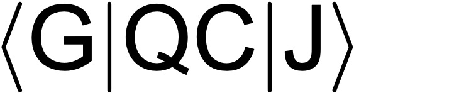
\includegraphics[height=30pt]{head_foot/journal_name}\hfill\raisebox{0pt}[0pt][0pt]{
\includegraphics[height=55pt]{head_foot/RSC_LOGO_CMYK}}\\[1ex]
      
\includegraphics[width=18.5cm]{head_foot/header_bar}}\par
    \vspace{1em}
    \sffamily
    \begin{tabular}{m{4.5cm} p{13.5cm} }

                     & \noindent\LARGE{\textbf{\ce{H3} as an Example for Open Shell systems: CIS with UHF and CUHF references.}} \\%Article title goes here instead of the text "This is the title"
      \vspace{0.3cm} & \vspace{0.3cm}                                                                                            \\

                     & \noindent\large{Ruben Van der Stichelen$^{\ast}$\textit{$^{a}$}}                                          \\%Author names go here instead of "Full name", etc.

                     &                                                                                                           \\

                     & \noindent\normalsize{}                                                                                    \\%The abstrast goes here instead of the text "The abstract should be..."
    \end{tabular}

  \end{@twocolumnfalse} \vspace{1.6cm}

]
%%%END OF TITLE, AUTHORS AND ABSTRACT%%%

%%%FONT SETUP - please do not change any commands within this section
\renewcommand*\rmdefault{bch}\normalfont\upshape
\rmfamily
\section*{}
\vspace{-1cm}


% %%%FOOTNOTES%%%

\footnotetext{\textit{$^{a}$~Ghent Quantum Chemistry Group, Krijgslaan 281 (S3), B-9000 Gent, België}}

% %Please use \dag to cite the ESI in the main text of the article.
% %If you article does not have ESI please remove the the \dag symbol from the title and the footnotetext below.
% \footnotetext{\dag~Electronic Supplementary Information (ESI) available: [details of any supplementary information available should be included here]. See DOI: 00.0000/00000000.}
% %additional addresses can be cited as above using the lower-case letters, c, d, e... If all authors are from the same address, no letter is required

% \footnotetext{\ddag~Additional footnotes to the title and authors can be included \textit{e.g.}\ `Present address:' or `These authors contributed equally to this work' as above using the symbols: \ddag, \textsection, and \P. Please place the appropriate symbol next to the author's name and include a \texttt{\textbackslash footnotetext} entry in the the correct place in the list.}


%%%END OF FOOTNOTES%%%

%%%MAIN TEXT%%%%


\section{Introduction}

\paragraph*{}
In computational chemistry, the time-independent Schrödinger equation plays a central role.

\begin{equation}\label{eq:erwin}
  \hat{H}\Psi = E\Psi
\end{equation}

All the information with regard to a certain molecule are linked to the wave function $\Psi$.
This information must be gathered using quantum mechanical operators. In the Schrödinger equation we
calculate this wave functions energy $E$ using an operator known as the Hamiltonian. In its full form it can be seen in the equation below\cite{Szabo1996}.

\begin{equation}\label{eq:ham}
  \hat{H} = -\sum_{i=1}^N\frac{1}{2}\nabla^2_i - \sum_{A=1}^M \frac{1}{2M_A}\nabla^2_A - \sum_{i=1}^N\sum_{A=1}^M\frac{Z_A}{r_{iA}} + \sum_{i=1}^N\sum_{j>i}^N\frac{1}{r_{ij}} +
  \sum_{A=1}^M\sum_{B>A}^M\frac{Z_A Z_B}{R_{AB}}
\end{equation}

The Hamiltonian contains the kinetic energy of the $N$ electrons $i$ and the $M$ nuclei $A$. It also accounts for the electrostatic potential between the nuclei and the electrons.
Also note that this Hamiltonian was written down using atomic units. Unfortunately, the Schrödinger equation is not exactly solvable for systems that contain more than one electron, i.e.
almost all chemically interesting systems. The reason for this is the repulsion that exists between two electrons. This term makes it impossible to solve the Schrödinger equation
analytically for most systems. That is why we need to make approximations. In this paper, we will make use of the Hartree-Fock method
combined with Single Excitation Configuration Interaction. In the Hartree Fock method, we use a single Slater determinant wave function that is an eigenfunction of the Fock
operator\cite{Szabo1996}.

\begin{equation}
  \hat{f} = \hat{h}(1) +  \sum_j^N \hat{J}_j - \hat{K}_j
\end{equation}

The operators $\hat{J}_j$ and $\hat{K}_j$ are called the Coulomb and exchange operators respectively. The Coulomb operator accounts for interelectronic repulsion, while the exchange
operator accounts for the stabilization that occurs between electrons of the same spin. \\

We can define an expectation value over the Hamiltonian and state that if we are in an energy minimum, a small variation in the wave function will not induce a change
in energy.

\begin{equation}\label{eq:hamexp}
  \langle\psi + \delta\psi|\hat{H}|\psi + \delta\psi \rangle = E + \delta E + \delta E^* + \delta E^2
\end{equation}

In first order we say that if the energy of the wave function $\psi$ is a minimum the wave function can be varied slightly without changing the expectation value over the
Hamiltonian, so $\delta E = 0$.
This approximation might take us a long way in the right direction, but does it take us all the way there? Here we need to introduce different methods within the
Hartree-Fock theory. Restricted Hartree-Fock (RHF) forces the electrons into the same orbitals, thus creating doubly occupied orbitals. Even though this is a valid picture
in organic chemistry, since we think about electrons in pairs, physically there is no obligation for the electrons to exist in these pairs.
When we let go of the restriction, we enter the Unrestricted Hartree-Fock method (UHF). This  is no longer confined to closed shell species since it has no problem with
electrons that do not exist in pairs. However, we see that the wave function in this method does not contain the right symmetries. We can get to a lower energy since we give
the wave function some extra freedom, yet the chemical intuition is tossed out of the window.
\paragraph*{}
A molecule can have a lot of symmetry elements, simple examples could be rotational axes or mirror planes. This symmetry is reflected in that molecules Hamiltonian and its wave
function.
Looking back at equation \eqref{eq:hamexp} and
the constraint we applied, namely that $\delta E$ should remain zero, we cannot state that our approximative Hartree-Fock wave function still abides by these symmetries.
We can impose some additional constraints in order to get the right symmetries, but there is a cost involved. This leads us to Löwdin's symmetry dilemma \cite{Lowdin1963}.
On one side we can enforce the symmetry. This will lead us to a wave function that is chemically intuitive, but the energy we reach will be relatively high. We can also expect to
keep the quantum numbers, such as $S$, associated with the wave function. On the other hand we can drop the symmetry. This will lead us to a lower energy wave function, but we will
lose information about the spin quantum numbers.

\paragraph*{}
We need some kind of theory to bring the best of both worlds together. On one side, we have the chemical intuition in the restricted wave functions, on the other the lower
energy in the unrestricted wave functions. Roothaan's Restricted Open Shell theory (ROHF)\cite{Roothaan1960} was an early attempt. As this approach is tedious and hard to implement,
it is not very popular\cite{Scuseria2010, Bally2008}. One of the drawbacks in ROHF method is that the Fock operator is not unambiguously defined\cite{Scuseria2010, Plakhutin2014}.
UHF is rather easy to implement \cite{Scuseria2010, Bally2008}, but as we stated above, there is a cost to this method.
However, more recently Tsuchimochi and Scuseria presented their Constrained Unrestricted Hartree-Fock theory (CUHF)
\cite{Scuseria2010}. In CUHF we apply a constraint to the system that sets the spin contamination to zero (cfr. infra). This is because spin contaminated wave functions are no
good starting point for post Hartree-Fock methods\cite{Scuseria2010}. A lot has been said
already about this method; Scuseria and Tsuchimochi themselves expanded on it in a follow-up paper\cite{Scuseria2011}. Plakhutin and Davidson discussed some defects in the theory
with respect to
Koopmans theorem and ionisations\cite{Plakhutin2014}. In this work we will use the CUHF wave function as a reference for
Single Excitation Configuration Interaction (CIS). We will generate the single excitation energies for the CUHF wave function and compare them to the CIS excitation energies using
ROHF and UHF references of the same system.
\paragraph*{}
In this work we will start by introducing spin-contamination and the theory behind it. We will also give an overview of CUHF theory. Then we will discuss CIS and derive some important
equations. Next we will look at spin-contamination in an actual system to stress the importance of uncontaminated spin. Then we will discuss the CIS results for CUHF, ROHF and UHF.
\section{Theory}
\subsection{Spin-Contamination}
\label{subsec:spinconttheory}
In general one can define the expectation value of $\hat{S}^2$ like equation \eqref{eq:spinexp}\cite{Andrews1991}.

\begin{equation}\label{eq:spinexp}
  \langle \hat{S}^2 \rangle = S_z^2 + S_z + q - \sum_{ij}^{pq} S_{ij}^2
\end{equation}

This equation is written down for a system with $p$ $\alpha$ electrons with summation index $i$ and $q$ $\beta$ electrons with summation index $j$. The $S$ matrix contains the overlap
between orbitals in the Molecular Orbital (MO)
basis. $S_z$ is the eigenvalue of the $\hat{S}_z$ operator. When the overlap is diagonal in this MO basis, the last two terms vanish, and we are left with $S_z(S_z + 1)$.
Spin-contamination is then defined as equation \eqref{eq:spincont}.

\begin{equation}\label{eq:spincont}
  \delta_s = \langle S^2 \rangle - S_z(S_z + 1)
\end{equation}

In UHF the overlap is not diagonal, so the overlap matrix between the $\alpha$ and $\beta$ orbitals will not be diagonal. One can not
expect the last two terms in equation \eqref{eq:spinexp} to vanish, which will result in $\delta_s$ not being equal to zero. This also means that the wave function is no longer an
eigenfunction of $\hat{S^2}$, as we have seen before. We lose a quantum number and with it the symmetry of the system. We can rewrite spin-contamination as equation
\eqref{eq:spincont2}\cite{Savin2010}.

\begin{equation}\label{eq:spincont2}
  \delta_s = N_\beta - Tr(\gamma^\alpha\gamma^\beta)
\end{equation}

In this equation, $\gamma^{\alpha}$ and $\gamma^\beta$ are the one particle density matrices. In the Natural Orbital (NO) basis, these matrices are block diagonal
\cite{Scuseria2010}, with blocks that can be seen in equations \eqref{eq:gammaa} and \eqref{eq:gammab}, where $i$ corresponds to a certain closed shell orbital. When there are more
$\alpha$ electrons than $\beta$ electrons,
the $\gamma^\alpha$ also contains a block that is a unity matrix with dimensions $n\times n$ where $n$ is the amount of singly occupied orbitals. In $\gamma^\beta$ this block is a
zero matrix of the same dimensions. For clarity, we will always assume that the amount of $\alpha$ electrons is larger than the amount of $\beta$ electrons. The results hold for any system
where $N_a \geq N_b $ \cite{Scuseria2010}.

\begin{subequations}
  \begin{align}
    \label{eq:gammaa}
    \gamma^\alpha_i & = \begin{bmatrix}
      n_i & m_i    \\
      m_i & 1- n_i
    \end{bmatrix}  &  & \\
    \label{eq:gammab}
    \gamma^\beta_i  & = \begin{bmatrix}
      n_i  & -m_i  \\
      -m_i & 1-n_i
    \end{bmatrix} &  &
  \end{align}
\end{subequations}

These matrices can now be written in their full form, as can be seen in equations \eqref{eq:gammaafull} and \eqref{eq:gammabfull}

\begin{subequations}
  \begin{align}
    \label{eq:gammaafull}
    \mathbf{\gamma}^\alpha = \begin{bmatrix}
      \gamma^\alpha_1 & \cdots & 0                      & 0      & 0      \\
      \vdots          & \ddots & \vdots                 & \vdots & \vdots \\
      0               & \cdots & \gamma^\alpha_{N_{cp}} & 0      & 0      \\
      0               & \cdots & 0                      & I_n    & 0      \\
      0               & \cdots & 0                      & 0      & 0
    \end{bmatrix} &  & \\
    \label{eq:gammabfull}
    \mathbf{\gamma}^\beta = \begin{bmatrix}
      \gamma^\beta_1 & \cdots & 0                     & 0      & 0      \\
      \vdots         & \ddots & \vdots                & \vdots & \vdots \\
      0              & \cdots & \gamma^\beta_{N_{cp}} & 0      & 0      \\
      0              & \cdots & 0                     & 0      & 0      \\
      0              & \cdots & 0                     & 0      & 0
    \end{bmatrix}  &  &
  \end{align}
\end{subequations}

$I_n$ is noted as the unity matrix in $n$ dimensions, where $n$ is the number of unpaired electrons. We have $N_{cp}$ closed shell orbitals, each corresponding with a doubly occupied
orbital. In our assumption that there are more $\alpha$ electrons than $\beta$ electrons, $N_{cp}$ is also equal to the amount of $\beta$ electrons.
In these equations $n_i$ is the occupation of orbital i and $m_i = \sqrt{n_i - n_i^2}$\cite{Scuseria2010}. We can then define the spin density matrix
$M = (\gamma^\alpha - \gamma^\beta)/2$. The matrix subtraction leaves us with blocks in the $M$ matrix that correspond to equation \eqref{eq:mmatrix}.

\begin{equation}\label{eq:mmatrix}
  M_i = \begin{bmatrix}
    0   & m_i \\
    m_i & 0
  \end{bmatrix}
\end{equation}

Of course, the open shell block will now consist of $\frac{1}{2}I_n$. Using this information we can rewrite equation \eqref{eq:spincont2} to equation
\eqref{eq:spincont3}\cite{Scuseria2010}.

\begin{equation}\label{eq:spincont3}
  \delta_s = N_\beta - (N_\alpha + N_\beta)/2 + 2*Tr(M^2)
\end{equation}

We can indeed verify that this is true by working out the matrix product as was done in proof \ref{proof1}.

\begin{proof}[Proof \ref{proof1}]\label{proof1}
  To a system with $N_e$ electrons of which $2N_{cp}$ are in the closed shell and $N_s$ are in the open shell applies:
  \begin{align*}
    Tr(\gamma^\alpha\gamma^\beta) & = \sum^{N_{cp}}_i (-4m_i + 1)               \\
                                  & = N_{cp} - \sum^{N_{cp}}_i 4m_i             \\
                                  & = \frac{N_e - N_s}{2} -\sum^{N_{cp}}_i 4m_i \\
                                  & = \frac{N_e}{2} - 2Tr(M^2)
  \end{align*}
\end{proof}

In an additional step, we can use algebra to find equation \eqref{eq:spincontfinal}. This equation can also be derived from proof \ref{proof1}.

\begin{equation}\label{eq:spincontfinal}
  \delta_s = 4\sum^{N_{cp}}_i m_i^2
\end{equation}

Now if we want to make the spin contamination zero, we have to enforce double occupation or no occupation at all. We see here that in
the closed shell itself, we can no longer have a difference between $\alpha$ and $\beta$ orbitals. This will be the constraint that gives us the CUHF method. We could make the observation
that in Roothaan's original paper, the start was very similar, as can be seen in equation \eqref{eq:rohfwf}\cite{Roothaan1960}.

\begin{equation}\label{eq:rohfwf}
  \Phi = (\phi_C,\phi_O)
\end{equation}

Roothaan starts his exposition on open shell systems with this equation, representing the total wave function $\Phi$ as a combination of a closed shell system $\phi_C$ and
an open shell system $\phi_O$

\subsection{Constrained Unrestricted Hartree-Fock}
\label{subsec:cuhftheory}
When talking about CUHF, there is more than one way to make sure that the spin-contamination remains zero. Scuseria and Tsuchimochi will enforce the constraint in the way
we mentioned in the last section, where they allow only doubly occupied orbitals in the closed shell\cite{Scuseria2010}. It can be shown that the normal UHF energy can be
constructed by adding a correlation energy term to the closed shell energy. These terms can be seen in equations \eqref{eq:cseng} and \eqref{eq:correng}\cite{Savin2010}.

\begin{subequations}
  \begin{align}
    \label{eq:cseng}
    E_{cs} & = 2\sum_{ij}h_{ij}P_{ij} + \sum_{ijkl}(2\langle ij|kl\rangle - \langle ij|lk \rangle)P_{ik}P_{jl} &  & \\
    \label{eq:correng}
    E_c    & = -\sum_{ijkl}\langle ij|lk \rangle M_{ik}M_{jl}                                                  &  &
  \end{align}
\end{subequations}

Where the matrix $M$ is the spin density matrix (cfr. supra) and the $P$ matrix is the charge density matrix: $P = (\gamma^\alpha + \gamma^\beta)/2$. If we take the
derivative with respect to the density matrices we find equations \eqref{eq:der1} and \eqref{eq:der2}.

\begin{subequations}
  \begin{align}
    \label{eq:der1}
     &  & \frac{\partial E_{cs}}{\partial \gamma^\alpha_{ij}} & = \frac{\partial E_{cs}}{\partial \gamma^\beta_{ij}} = F^{cs}_{ij}                                             \\
    \label{eq:der2}
     &  & -\frac{\partial E_c}{\partial \gamma^\alpha_{ij}}   & = \frac{\partial E_c}{\partial \gamma^\beta_{ij}} = \sum_{kl} \langle ik|lj \rangle M_{kl} = \Delta^{UHF}_{ij}
  \end{align}
\end{subequations}

So in fact, the UHF Fock operators can be written as a sum of this $\Delta^{UHF}$ and the closed shell Fock operator, as displayed in equations \eqref{eq:uhfa} and \eqref{eq:uhfb}
\cite{Scuseria2010}.

\begin{subequations}
  \begin{align}
    \label{eq:uhfa}
    F^\alpha = F_{cs} - \Delta^{UHF} \\
    \label{eq:uhfb}
    F^\beta = F_{cs} + \Delta^{UHF}
  \end{align}
\end{subequations}

Now we need to expand this concept to CUHF. In general, we want
to be able to write the CUHF Fock matrix $\tilde{F}$ as the closed shell Fock matrix to which we add a certain $\Delta^{CUHF}$. As we have already seen, the constraint is only
applied to the virtual and closed shell orbitals. When we display the Fock matrix in MO basis it will exist in blocks, \eqref{eq:fockblock}. The \textit{c}, \textit{o} and \textit{v}
stand for closed shell, open shell and virtual respectively.

\begin{equation}\label{eq:fockblock}
  \mathbf{F} = \begin{bmatrix}
    F_{cc} & F_{co} & F_{cv} \\
    F_{oc} & F_{oo} & F_{ov} \\
    F_{vc} & F_{vo} & F_{vv} \\
  \end{bmatrix}
\end{equation}

We apply the constraint in the \textit{vc} and \textit{cv} blocks. We can do this by stating that $[\tilde{F}^\sigma, \gamma^\sigma] = 0$, where $\sigma$ can equal either $\alpha$
or $\beta$. This basically means that the density matrices should share a complete set of eigenfunctions with the Fock matrices. This, in turn, means that the Fock matrices should be
diagonal at self-consistent field (SCF) conditions in the NO basis. By subtracting the two conditions and algebraically working out the result we find that at SCF conditions
$\Delta^{CUHF}_{cv}$ has to be equal to zero. This means that $\tilde{F}_{cv} = F_{cv}^{cs}$\cite{Scuseria2010}. For every other block, the CUHF Fock matrix equals the UHF Fock matrix,
so the $\Delta^{CUHF}$ equals the $\Delta^{UHF}$. When we enforce this constraint during every iteration, we will decrease the spin contamination. This does entail that we will need
to transform the $\Delta^{UHF}$ to NO basis every time to enforce this constraint. This transformation will consist of two steps. First we need to transform the density matrix to
an orthonormal basis, since AO basis is often not orthonormal. (Indeed, if it were, we would not expect any bonds to form.) We choose MO basis. The MO's are defined by the
eigenvectors of the Fock operator, we will use the closed shell Fock operator. Given the Roothaan equation \eqref{eq:roothaan}.

\begin{equation}\label{eq:roothaan}
  F_{cs}C = \epsilon S C
\end{equation}

With a simple transformation, we can see that the Fock operator will become diagonal using the transformation in equation \eqref{eq:fmo}

\begin{equation}\label{eq:fmo}
  C^T F C = \epsilon C^T S C
\end{equation}

This is true, since $C^T S C$ it the unity matrix if the C matrix holds the eigenvectors of the generalized eigen value problem. To transform to NO basis, we will also need the
density matrix in the MO basis. This is not trivial, since the density matrix is usually defined by the coefficient matrices C. To transform the density matrix $P$, we will need
to do a slightly different transformation. This transformation is given in equation \eqref{eq:dtrans}\cite{Declercq2020}.

\begin{equation}\label{eq:dtrans}
  P^{MO} = C^{-1}P^{AO}(C^{-1})^T
\end{equation}

We can then calculate the eigenvalues and subject the $\Delta^{UHF}$ to these transformations \eqref{eq:fulltrans}, we have easy access to the \textit{cv} and \textit{vc} blocks.

\begin{equation}\label{eq:fulltrans}
  \Delta_{NO}^{UHF} = V^{-1} C^T \Delta^{UHF}_{AO} C V^{-1}
\end{equation}

The $V$ matrix contains the coefficients of the eigenvectors of the $P$ matrix. Now we just switch the required blocks to zero, back transform and add the now $\Delta$ to the closed
shell Fock matrix. To summarize this procedure we can look at the form of the Fock matrices in equations \eqref{eq:cuhfa} and \eqref{eq:cuhfb}.

\begin{subequations}
  \begin{align}
    \label{eq:cuhfa}
    \tilde{F}^\alpha = F_{cs} - \Delta^{CUHF} \\
    \label{eq:cuhfb}
    \tilde{F}^\beta = F_{cs} + \Delta^{CUHF}
  \end{align}
\end{subequations}

Where $\Delta^{CUHF}$ is either zero or $\Delta^{UHF}$ depending on whether you are looking at the \textit{cv} blocks or at the other blocks. Here we can also clearly see the
difference with ROHF theory. In his original paper, Roothaan goes through great lengths to ensure that there is only one Fock matrix instead of separate ones for the $\alpha$ and
$\beta$ orbitals\cite{Roothaan1960}. This makes it rather difficult to interpret results\cite{Scuseria2010}. However, Scuseria and Tsuchimochi keep the separate matrices, like in a
normal UHF approach. This means that we will end up with a slightly different picture from the ROHF picture, but the wave function and its energy remain the same\cite{Scuseria2010}.

\subsection{Configuration interaction}
\label{subsec:cistheory}

The Hartree-Fock approximation gives us an initial guess for the energy and the wave function. However, it can be improved upon. The methods that do this are called post Hartree-Fock
methods. The difference in energy between the normal Hartree-Fock method and the post Hartree-Fock method is called the correlation energy \eqref{eq:Ecorr}.

\begin{equation}\label{eq:Ecorr}
  E_{corr} = \mathcal{E}_0 - E_0
\end{equation}

Here $E_0$ is the Hartree-Fock energy and $\mathcal{E}_0$ it the post Hartree-Fock energy. There are various approaches to post Hartree-Fock methods. We will discuss the
Configuration Interaction method(CI).
If $\Phi_0$ is the result of normal Hartree-Fock procedure, it is an approximation of the true wave function $\Gamma$. We know that we can make a better approximation
using a linear combination of excited states that start from $\Phi_0$\cite{Szabo1996}. If $\Phi_0$ is the Slater determinant that corresponds to the ground state of the system, we
mix it with the excited states. Each determinant represents a certain configuration of the electrons. These configurations interact, as can be seen in the equation below.

\begin{equation}\label{eq:lincomb}
  |\Psi_0\rangle = c_0|\Phi_0\rangle + \sum_{ar}|\Phi_a^r\rangle + \sum_{a<b,r<s}c_{ab}^{rs}|\Phi^{rs}_{ab} \rangle + \cdots
\end{equation}

This wave function $\Psi_0$ is a better approximation to the real wave function $\Gamma$ than $\Phi_0$. When we try to get the energy expectation value of this function, we can write
it in matrix form, where each row and column correspond to a certain excited state. The full expression of this matrix is given below.

\begin{equation}\label{eq:hamexp1}
  \mathbf{H} = \begin{bmatrix}
    \langle \Phi_0 | \hat{H} | \Phi_0 \rangle                         & \langle \Phi_0 | \hat{H} | \Phi_r^a \rangle   & \cdots & \langle \Phi_0 | \hat{H} | \Phi_{\{\chi_o\}}^{\{\chi_v\}} \rangle \\
    \langle \Phi_r^a | \hat{H} | \Phi_0 \rangle                       & \langle \Phi_r^a | \hat{H} | \Phi_r^a \rangle & \cdots & \langle \Phi_r^a | \hat{H} | \Phi_{\{\chi_o\}}^{\{\chi_v\}} \rangle \\
    \vdots                                                            & \vdots                                        & \ddots & \vdots                                                                                    \\
    \langle \Phi_{\{\chi_o\}}^{\{\chi_v\}} | \hat{H} | \Phi_0 \rangle & \cdots                                         & \cdots & \langle \Phi_{\{\chi_o\}}^{\{\chi_v\}} | \hat{H} | \Phi_{\{\chi_o\}}^{\{\chi_v\}} \rangle
  \end{bmatrix}
\end{equation}

For a system with $n$ occupied orbitals in the ground state, denoted with indices $(r, s)$ and $m$ unoccupied orbitals, denoted with indices $(a,b)$, the full CI matrix extends until
every possible electron configuration has been accounted for. $\Phi_{\{\chi_o\}}^{\{\chi_v\}}$ is a state in which a set of $m$ electrons is excited. In the ground state, these
electrons occupy the set of orbitals {$\chi_o$}, and they are excited to the set of virtual orbitals {$\chi_v$}.
We now have to determine what all the different matrix elements are. Since we are looking at CIS, we are only interested in the single excitations, so the matrix in equation
\eqref{eq:hamexp1} can be simplified quite a bit. All elements that contain a higher order excitation are set to zero. Then we already know that the expectation value of the Hartree-Fock wave function is the energy we can get from our normal
Hartree-Fock calculation, so we can write this equation.

\begin{equation}\label{eq:E0}
  \langle \Phi_0 | \hat{H} | \Phi_0 \rangle = E_0
\end{equation}

When we look at single excitations, so at states $\Psi_r^a$ where the electron from orbital $r$ has been excited to orbital $a$, we can write equation
\eqref{eq:overlapsingle}\cite{Szabo1996} for the overlap between the ground state wave function and the excited states.

\begin{equation}\label{eq:overlapsingle}
  \langle\Phi_0 |\hat{H}|\Phi_r^a\rangle = \langle a|h|r \rangle + \sum_b \langle ab||rb \rangle = \langle \chi_a |\hat{f}| \chi_r \rangle = F_{ra}
\end{equation}

Here $\langle ab||rb \rangle$ is shorthand notation for $\langle ab | rb \rangle - \langle ab | br \rangle$. The letter $a$ represents the orbital $\chi_a$.
Now of course, by definition, at SCF conditions the off-diagonal elements of the Fock matrix are zero. This leads to Brillouin's theorem. It states that there is no overlap
between single excited states and the ground state wave function when taking the expectation value over the Hamiltonian. This means that the ground state energy cannot be improved
upon by doing a CIS calculation. Indeed, one can prove equation \eqref{eq:doubles}\cite{Szabo1996}. The correlation energy is only defined by the overlap between second order
excited states.

\begin{equation}\label{eq:doubles}
  E_{corr} = \sum_{i<j, r<s} C_{ij}^{rs}\langle \Phi_{0} |\hat{H}|\Phi_{ij}^{rs}\rangle
\end{equation}

However, this does not mean that an excited state can not have a lower energy than the ground state. This can be understood by looking again at equation \eqref{eq:hamexp} and only
considering columns and rows that contain the ground state or a single excitation. What we have now is in fact a block diagonal matrix. One block contains the ground state energy, so
its dimensions are $1\times 1 $. The other block contains all the excited state expectation values and overlap elements. It is a property of block diagonal matrices that their
eigenvalues are the eigenvalues of the individual blocks. We can thus conclude that the ground state energy will be among the eigenvalues of this matrix. There is nothing that
constrains the eigenvalues of the other block, so they might well be lower than the ground state energy. One can imagine a situation where the geometry of the molecule has not been
optimized, in which it might be favorable to be in an excited state rather than in the ground state.

In CIS, we do not expect to lower the ground state energy. However, it can give us information about the
excited states and the excitation energies that come with them. Now we are interested in the expectation values over the Hamiltonian of all the exited states, so we need an expression
for $\langle \Phi_r^a |\hat{H}| \Phi_s^b \rangle$. There are four different situations that we need to discuss here\cite{Sherrill1996}. The first scenario is an excitation where
$a \neq b$ and $r \neq s$. The only term that will remain in that case is $\langle aj || ib \rangle$. Another case is when $r = s$ but $a \neq b$. Then the matrix element can be
expressed using equation \eqref{eq:exp1}.

\begin{equation}\label{eq:exp1}
  \langle \Phi_r^a|\hat{H}|\Phi^b_r \rangle = h_{ab} + \sum_{k\in r} \langle ak || bk \rangle = F_{ab} - \langle ar||br \rangle
\end{equation}

Another case, where $r \neq s$ and $a = b$ we can write equation \eqref{eq:exp2}.

\begin{equation}\label{eq:exp2}
  \langle \Phi_r^a|\hat{H}|\Phi^a_s \rangle = -h_{rs} - \sum_{k \in \{\Psi_0 + a\}} \langle ak || bk \rangle = -F_{rs} - \langle ra || sa \rangle
\end{equation}

Finally, when both $a = b$ and $r = s$ we can find equation \eqref{eq:exp3}.

\begin{multline}\label{eq:exp3}
  \langle \Phi^a_r|\hat{H}|\Phi^a_r \rangle = \sum_{k \in \Psi_0}h_{kk} + \frac{1}{2}\sum_{k,l \in \Phi_0} \langle kl||kl \rangle - h_{rr} + h_{aa} \\ - \sum_{k \in \Phi_0} \langle
  kr || kr \rangle + \sum_{k \in \Phi_0} \langle ka||ka \rangle - \langle ra||ra \rangle
\end{multline}

We can pull all these equations into one general equation \eqref{eq:matrixelement}.

\begin{equation}\label{eq:matrixelement}
  \langle \Phi_r^a|\hat{H}|\Phi_s^b \rangle = E_0\delta_{rs}\delta_{ab} + F_{ab}\delta_{rs} - F_{rs}\delta_{ab} + \langle as || jb \rangle
\end{equation}

We notice that $E_0$ is added along the diagonal. Since we know that the trace of a matrix is equal to the sum of its eigenvalues, we can subtract $E_0$ from the diagonal and just
add it to every eigenvalue at the end. At self-consistent field conditions the Fock operator equals $F_{ij} = \epsilon_i\delta_{ij}$, so equation \eqref{eq:matrixelement} can be
simplified to equation \eqref{eq:simple}.

\begin{equation}\label{eq:simple}
  \langle \Phi_r^a|\hat{H}|\Phi_s^b \rangle = (\epsilon_a - \epsilon_r)\delta_{rs}\delta_{ab} + \langle as || jb \rangle
\end{equation}

The $\epsilon_i$ values correspond to the orbital energies. If we now diagonalize the CIS matrix we end up with the excitation energies and contributions of the single excited states as
eigenfunctions. However, since electrons in $\alpha$ orbitals can be excited to $\beta$ orbitals, which is especially important in UHF, we have to do some extra steps. Indeed, when
calculating the eigenfunctions of the Fock matrices we get separate coefficient matrices for $\alpha$ and $\beta$ orbitals. We will need all these orbitals together to get the complete
CIS picture. We will have to effectively double the dimensions of the problem. This becomes a bit clearer by looking at equation \eqref{eq:matrixelement}. In this equation for example
$a$ and $b$ do not have the same spin. However, the expression $F_{ab}$ implies that there is an overlap element in the Fock matrix between two orbitals that can have a different spin.
We can see that the normal $\alpha$ and $\beta$ Fock matrices will not be enough. We will need a Fock matrix that accounts for both $\alpha$ and $\beta$ electrons, and has the respective orbitals
as eigenfunctions. A block diagonal matrix like equation \eqref{eq:blockfock} is a logical choice. Its eigenvalues will be the combination of the sets of eigenvalues of the blocks,
the same goes for its eigenvectors.

\begin{equation}\label{eq:blockfock}
  F = \begin{bmatrix}
    F^\alpha & 0       \\
    0        & F^\beta
  \end{bmatrix}
\end{equation}

When looking at equation \eqref{eq:matrixelement} we see that we also need the so-called two electron integrals. This is in fact a four dimensional matrix that holds the
interelectronic repulsion in AO basis. We also need to double its dimensions in order to use it for CIS calculations. Since this is an $n\times n\times n \times n$
matrix, we will need to use the Kronecker product.

\begin{equation}\label{eq:kron}
  R' = I_2 \otimes (I_2 \otimes R)^T
\end{equation}

The $R'$ matrix now has double the dimensions of the original R matrix. R in this case is the two electron overlap matrix. This is necessary for the two electron integrals, since
they only contain half the orbitals. These integrals are in the original basis, but we need to account for all possible excitations, meaning that we have to account for alpha and
$\beta$ orbitals at the same time. Since the two electron integrals are given in AO basis, they still need to be transformed to MO basis, since we want the Fock operators to be
diagonal in equation \eqref{eq:matrixelement}. To do this transformation we will need the coefficient matrix that holds the eigenfunction of the matrix in equation
\eqref{eq:blockfock}.

\section{Methodology}
\label{sec:method}
The RHF, UHF and CUHF algorithms were self-implemented. The following iterative algorithm was applied for (C)UHF:
\begin{enumerate}
  \item Calculate the energy based on the current guess matrices (the core Hamiltonian for the first iteration). There is a different guess matrix for $\alpha$ and $\beta$ electrons.
  \item Calculate a new Fock matrix for both $\alpha$ and $\beta$ electrons based on the eigenfunctions of the current guess matrices.
  \item In CUHF we now manipulate the Fock matrices as described in the \ref{subsec:cuhftheory} section. In UHF this step is skipped
  \item Set the new Fock matrices as new guess matrices.
  \item Check for convergence. This was done using an energy criterion with a threshold of $10^{-12}$ Hartree.
\end{enumerate}

The CIS algorithm was implemented using equation \eqref{eq:simple} to create the Hamiltonian matrix elements. Then a block was added containing only the expectation value of the
reference. The matrix was then diagonalized.
We used the packages NumPy\cite{Numpy}, SciPy\cite{Scipy} and Psi4\cite{Psi4}. NumPy and SciPy deliver tools for matrix manipulation
and other linear algebra calculations that we had to do. Psi4 is an open source quantum chemistry package allows us to calculate certain properties of the system given a molecular
geometry. These properties include nuclear repulsion, kinetic energy of the electrons among others. It also allows us to generate reference data for the molecular energy in RHF, UHF
and CUHF. It also features a method for calculating ROHF energies. They also present the possibility to do configuration interaction for RHF and ROHF. The CIS reference data for
UHF and CUHF were generated using the GQCP\cite{GQCP} library. We have also visualized some orbitals using Psi4's \lstinline{cubeprop} function to generate a .cube file. This .cube
file was then visualized using the IQmol software\cite{IQmol}.
\paragraph*{}
To demonstrate the impact of spin contamination and the importance of finding methods to overcome it, we will discuss the hydrogen gas dissociation problem\cite{Szabo1996}. Hydrogen
gas is a molecule that has an RHF solution in its equilibrium geometry. However, when we stretch the bond the system evolves to a state of separate hydrogen atoms. 
For CIS \ce{H3} will be used as a model system. Firstly because it is a simple system containing few electrons. This means that we do not need to track a lot of possible excitations,
so the focus can shift towards the interpretation. For this same reason we will pick the STO-3G basis set. This set provides us with the minimal amount of basis functions needed to
describe the system. This again makes interpretation the key point. We will also do a stretch of \ce{H3} in the following way. Since the molecule is an equilateral triangle, 
we will stretch all the bonds equally. Then we will compare the CIS results for \ce{H3} as generated by our implementation and the one used by Psi4 and GQCP.
GQCP will generate the data for CUHF and UHF and Psi4 will generate the data for ROHF.

\section{Results and discussion}
\label{sec:results}

\subsection{\ce{H2} Stretch}
\label{subsec:h2}
In figure \ref{fig:rhfstretch} we have conducted a stretch of the \ce{H2} molecule using an RHF calculation.
\begin{center}
  \begin{figure}[h]
    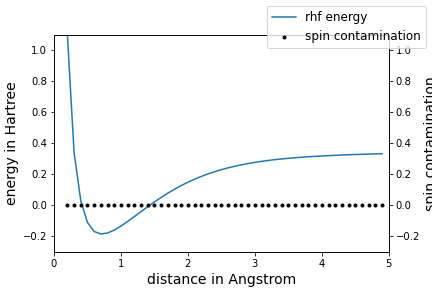
\includegraphics[width=\linewidth]{./../notes/figures/rhf.png}
    \caption{The RHF energy against the distance in an \ce{H2} stretch. The zero level was chosen as the energy of two separate hydrogen atoms.}
    \label{fig:rhfstretch}
  \end{figure}
\end{center}
We can see that the RHF energy does not behave as we would expect it to. Indeed, we expect the energy to evolve towards the energy of two separate hydrogen atoms, which clearly does
not happen. This is because the physical picture we are seeing is intrinsically invalid. The RFH algorithm forces the electrons into the same orbital, the bonding orbital between
the two nuclei. However, when the bond length increases, we expect the electrons to each be in their own respective orbitals around a single nucleus. At a distance of infinity, they
should find themselves in a normal hydrogen s orbital. The RHF description is too limited and does not allow this. Worth noting is that the spin contamination remains zero all the 
way. This means that the wave function is an eigenfunction of the $\hat{S}^2$\cite{Scuseria2011}. \\

We want to improve this image by using UHF.  When we drop the constraint that the $\alpha$ and $\beta$ orbitals must be identical we can indeed expect the energy to behave like we expect
it to. But since \ce{H2} is a closed shell system we need to do a little manipulation before starting the algorithm. When we would do a core guess, so start from the molecular
Hamiltonian as an approach for two Fock matrices, we would still find the restricted solution. To counteract this we will need to start from a mixed guess. For this we change the initial
guess for the $\beta$ electrons by mixing the Highest Occupied Molecular Orbital (HOMO) and the Lowest Unoccupied Molecular Orbital (LUMO) as a linear combination. This process is also
known as orbital mixing. The result can be seen in \ref{fig:uhfstretch}.
\begin{center}
  \begin{figure}[h]
    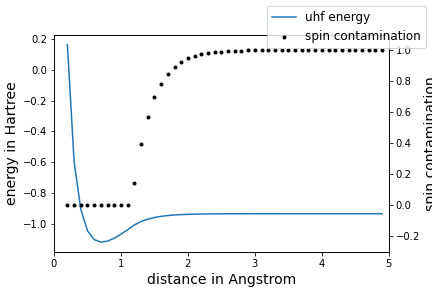
\includegraphics[width=\linewidth]{./../notes/figures/uhf.png}
    \caption{The UHF energy against the distance in an \ce{H2} stretch.}
    \label{fig:uhfstretch}
  \end{figure}
\end{center}
This result is physically more accurate. We see that the system does evolve towards two separate hydrogen atoms. However, the spin contamination is rising, and after a certain point
reaches the value one. This means that the wave function does no longer have the right symmetry. And as stated before, even if we cannot calculate the exact wave function we do know
what symmetries it should have. Even though we might have a lower energy, the wave function is not as good as an approximation as it could be\cite{Scuseria2013}. \\
This is a prime example of the aforementioned symmetry dilemma by Löwdin. If we want the lowest possible energy, we lose the symmetry. If we want to keep the symmetry, we will not
have the lowest energy. Now what would happen if we applied CUHF to the dissociation problem? This result has been plotted in figure \ref{fig:cuhfstretch}.
\begin{center}
  \begin{figure}[h]
    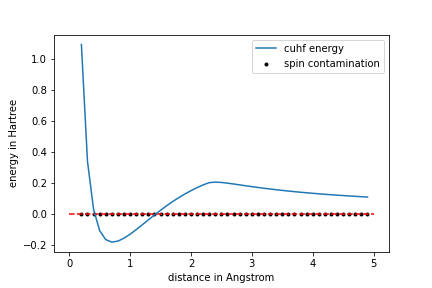
\includegraphics[width=\linewidth]{./../notes/figures/cuhf_mix.png}
    \caption{The CUHF energy against the distance in an \ce{H2} stretch.}
    \label{fig:cuhfstretch}
  \end{figure}
\end{center}
The CUHF picture is difficult to interpret. We see that the spin contamination remains zero, as can be expected. The energy seems to follow the RHF pattern (see also figure
\ref{fig:combo}) until a certain point, then it starts to exponentially decrease. Physically this seems like a logical behavior, as it is now again evolving to two separate hydrogen
atoms. We can also notice
that the spin contamination is zero everywhere, so the symmetry of the solution is also correct. For this plot a mixed guess was applied. In CUHF the mixed guess is done on the
active space, which consists the orbitals to which the constraints are not applied, i.e. the open shell\cite{Scuseria2011}. So when we would take the active space as all the electrons
we reach the UHF solution. When we take only unpaired electrons as the active space we see the ROHF solution.
\begin{center}
  \begin{figure}[h]
    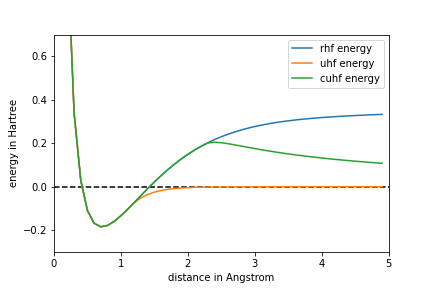
\includegraphics[width=\linewidth]{./../notes/figures/combo.png}
    \caption{The stretch energies plotted together.}
    \label{fig:combo}
  \end{figure}
\end{center}
For comparison, we plotted all the stretches in one plot, figure \ref{fig:combo}. Here we can see that they all describe short bond lengths correctly, but as the internuclear distance
increases, there are deviations visible. As one would expect, the CUHF energy is able to describe short bond lengths as correctly as both RHF and UHF. While RHF deviates from the
true physical value at long bond distances, we see that CUHF does follow the expected limits (going to zero at infinity) while keeping the symmetry intact. 

\subsection{\ce{H3} stretch}
\label{subsec:h3}
We will now discuss our model system, the trihydrogen molecule. This system is a ring of three hydrogen atoms, forming an equilateral triangle.
This system is an open shell system, as stated before, with two $\alpha$ electrons and one $\beta$ electron. It can not be described using RHF, since RHF needs closed-shell systems to work
properly. For UHF, we have plotted the result in figure \ref{fig:uhf_h3}.
\begin{center}
  \begin{figure}[h]
    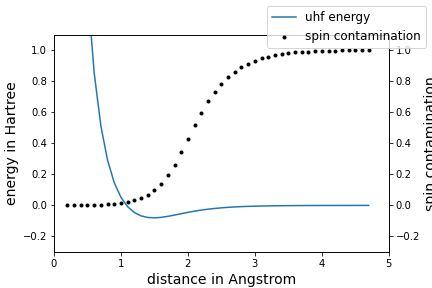
\includegraphics[width=\linewidth]{./../notes/figures/h3_uhf_sto-3g.png}
    \caption{The stretch for \ce{H3} using UHF.}
    \label{fig:uhf_h3}
  \end{figure}
\end{center}
We can see that the energy reaches the limiting case that we want, however the spin contamination is rising. In this figure, the last two data points were not plotted since convergence
could not be reached.  We can see that the molecule disintegrates into the three separate hydrogen atoms.
After that, the energy reaches the level of three separate hydrogen atoms. We can also take a look at the CUHF result in
figure \ref{fig:cuhf_h3}.
\begin{center}
  \begin{figure}[h]
    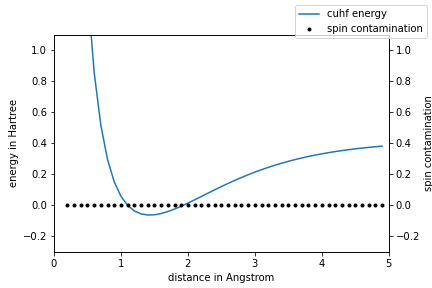
\includegraphics[width=\linewidth]{./../notes/figures/h3_cuhf.png}
    \caption{The stretch for \ce{H3} using CUHF.}
    \label{fig:cuhf_h3}
  \end{figure}
\end{center}
We can see that across the plotted data, the spin contamination remains zero. The curve is also smoother than the UHF curve. Where
the UHF curve might suggest a disintegration, the CUHF curve rises above the level of three separate hydrogens. When we consider the constraint we have introduced this is hardly
surprising. We have said that there are certain orbitals that have to be doubly occupied, as laid out in subsections \ref{subsec:spinconttheory} and \ref{subsec:cuhftheory}.
This is of course something we can not maintain at very long bondlenghts. Physically we could state that if we were to pull the hydrogen atoms apart far enough, they would go
their separate ways, since this would be the more energetically stable solution, instead of trying to maintain the bonds across such large distances. It is then reasonable that
the energy would rise as we continue to enforce this constraint.

\subsection{CIS results}
\label{subsec:cis}
In \ce{H3} we can consider nine excitations in total, so when we include the ground state, we should have ten states in total. We can take a closer look at
figure \ref{fig:h3_cis}.
\begin{center}
  \begin{figure}[h]
    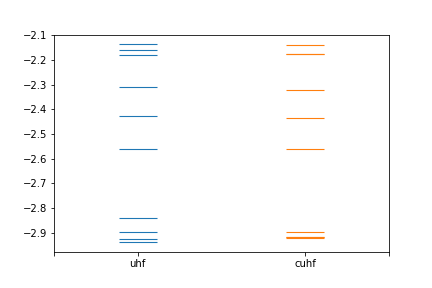
\includegraphics[width=\linewidth]{./../notes/figures/h3_cis.png}
    \caption{The CIS excitation energies for both UHF and CUHF as plotted by our implementation}
    \label{fig:h3_cis}
  \end{figure}
\end{center}
When we look at the UHF energies, we have ten distinct values. In CUHF we have some degeneracies in the excitation energy levels.
We can take a look at the table \ref{tab:excits}.
\begin{table}[h]
  \caption{The electronic excitation energies of \ce{H3} in STO-3G basis. The energy is given in Hartree.}
  \label{tab:excits}
  \begin{tabular}{l|l|l}
       & UHF       & CUHF      \\
    \hline
    1  & -2.938139 & -2.922658 \\
    2  & -2.923512 & -2.915707 \\
    3  & -2.896022 & -2.915707 \\
    4  & -2.840079 & -2.895707 \\
    5  & -2.560947 & -2.560947 \\
    6  & -2.428072 & -2.436524 \\
    7  & -2.309793 & -2.323014 \\
    8  & -2.179570 & -2.176621 \\
    9  & -2.160308 & -2.176621 \\
    10 & -2.137036 & -2.139049
  \end{tabular}
\end{table}
We do indeed notice that energies two and three are equal, as well as the energies eight and nine. Of course, it is logical to find a UHF result where all the expectation values are
different. If all orbitals are different, We can expect all energy differences to be different as well. However, in CUHF we discover that there are some identical
excitation energies. The reason is that the ground state and the mentioned excited state are degenerate. (cfr. infra)\\
We can also note another odd feature in both energies. The lowest excitation does not equal the ground state. When we consult our data in table
\ref{tab:ground states}, we notice that the lowest excitation is lower in energy than the ground state.
\begin{table}[h]
  \caption{Electronic ground state energies for \ce{H3} in the STO-3G basis. The energy is given in Hartree.}
  \label{tab:ground states}
  \begin{tabular}{l|l|l}
                        & UHF       & CUHF      \\
    \hline
    ground state energy & -2.923512 & -2.915707
  \end{tabular}
\end{table}
This data was verified using the GQCP library. This result is unexpected, since one does not expect an excitation to be lower in energy than the ground state. We could verify that
this excitation is a triplet excitation, or an excitation in which an $\alpha$ electron is excited to a $\beta$ orbital and vice versa. We could also determine the spin eigenvalue using
the GQCP library as 0.5, which means that it still is a spin eigenstate. A possible explanation could be that the ground state of \ce{H3} is degenerate, but in Hartree-Fock, we always 
take a single slater determinant into account. In fact, the ground state contains two determinants. When we mix the determinants in CIS, the result is a decreased energy.  
We can see these determinants in figure \ref{fig:energydiag1}Furthermore, we can learn from this that for open shell species that have spin
deficiencies, CIS is not the method of choice if we want to include the triplet excitations. When the triplet excitations are left out of the calculation, we find a result more
in line with our expectations, in which the ground state is the lowest energy state. These results were displayed in table \ref{tab:excits_no_triplets}\\
\begin{table}[h]
  \caption{The excitation energies when triplets are not considered. The energy is given in Hartree.}
  \label{tab:excits_no_triplets}
  \begin{tabular}{l|l|l}
      & UHF       & CUHF      \\
    \hline
    1 & -2.923515 & -2.915707 \\
    2 & -2.840101 & -2.895707 \\
    3 & -2.428086 & -2.436524 \\
    4 & -2.160319 & -2.176620 \\
    5 & -2.137039 & -2.139049
  \end{tabular}
\end{table}
We can also notice that the degeneracies have also disappeared, meaning that one of the excited states in both degeneracies was a triplet excitation. From the chemical point of view
this is logical. When we think of the \ce{H3} molecule in STO-3G basis, there are three orbital pairs to consider. Let us take a look at the orbital diagram in figure \ref{fig:energydiag1}.
\begin{figure}[h]
  \begin{center}
    \begin{tikzpicture}
      \draw (-1.25, 0.5) -- (-0.75, 0.5);
      \draw (-1.25, 0) -- (-0.75, 0);
      \draw (-1.25, -0.5) -- (-0.75, -0.5);
      \draw [-{Straight Barb[left]}] (-1.1, -0.60) -- (-1.1, -0.20);
      \draw [-{Straight Barb[left]}] (-1.1, -0.10) -- (-1.1, 0.30);
      \draw [-{Straight Barb[left]}] (-0.9, -0.20) -- (-0.9, -0.60);

      \draw (1.25, 0.5) -- (0.75, 0.5);
      \draw (1.25, 0) -- (0.75, 0);
      \draw (1.25, -0.5) -- (0.75, -0.5);
      \draw [-{Straight Barb[left]}] (0.9, -0.60) -- (0.9, -0.20);
      \draw [-{Straight Barb[left]}] (1.1, 0.30) -- (1.1, -0.10);
      \draw [-{Straight Barb[left]}] (1.1, -0.20) -- (1.1, -0.60);
    \end{tikzpicture}
  \end{center}
  \caption{Energy diagrams of the ground state of \ce{H3}}
  \label{fig:energydiag1}
\end{figure}
We can see in this picture that it does not make a difference what spin the unpaired electron has towards the energy. So in fact we expect to see a degeneracy at the ground state
energy level. Since this does involve an $\alpha$ to $\beta$ excitation we do not expect to see it when leaving those out. The other degeneracy was seen at the energy level of $-2.176620$
Hartree. We can consult GQCP in order to find the exact excitation that is done. The configuration is given in figure \ref{fig:energydiag2}.
\begin{figure}[h]
  \begin{center}
    \begin{tikzpicture}
      \draw (-0.25, 0.5) -- (0.25, 0.5);
      \draw (-0.25, 0) -- (0.25, 0);
      \draw (-0.25, -0.5) -- (0.25, -0.5);
      \draw [-{Straight Barb[left]}] (-0.1, -0.60) -- (-0.1, -0.20);
      \draw [-{Straight Barb[left]}] (-0.1, -0.10) -- (-0.1, 0.30);
      \draw [-{Straight Barb[left]}] (0.1, 0.80) -- (0.1, 0.40);
    \end{tikzpicture}
  \end{center}
  \caption{Energy diagram of the state at $-2.176620$ Hartree in CUHF}
  \label{fig:energydiag2}
\end{figure}
Based on this picture, we expect the same excitation energy if the $\alpha$ electron from $\psi_1$ would be excited. We can take a look at the orbitals in question.
They are displayed in figure \ref{fig:1_cuhf}.
\begin{figure}[h]
  \includegraphics[width=\linewidth]{./../notes/figures/H3_1_a.png}
  \includegraphics[width=\linewidth]{./../notes/figures/H3_1_b.png}
  \caption{$\psi_1$ for both $\alpha$ (top) and $\beta$ electrons (bottom)}
  \label{fig:1_cuhf}
\end{figure}
We detect some asymmetry in the orbitals. Normally we would expect \ce{H3} to be a $D_{3h}$ system. However, Psi4 has lowered the symmetry to a $C_{2v}$
point group. The reason for this is that it does not contain all possible point groups.
We will now compare the CIS data with CUHF reference to the CIS data with ROHF reference generated by Psi4.
The Psi4 reference data for ROHF generates two states, one of which is the ground state. The energies are given in table \ref{tab:ROHF}. Psi4 does not consider triplet excitations by
default, but we are still left with fewer excitations than one would expect.
\begin{table}[h]
  \caption{Electronic excitation energies of \ce{H3} in ROHF according to psi4. The energy is given in Hartree.}
  \label{tab:ROHF}
  \begin{tabular}{l|l}
      & energy    \\
    \hline
    1 & -2.915707 \\
    2 & -2.176621
  \end{tabular}
\end{table}
We can see that the ground state energy is the same as CUHF method. However, the single excitation can also be seen returning to the CUHF excitations. Psi4 lists the excitation it
considered as an excitation of the $\beta$ electron into the open shell, so if we were to draw it up using an energy diagram, it would look like figure \ref{fig:energydiag3}.
\begin{figure}[h]
  \begin{center}
    \begin{tikzpicture}
      \draw (-0.25, 0.5) -- (0.25, 0.5);
      \draw (-0.25, 0) -- (0.25, 0);
      \draw (-0.25, -0.5) -- (0.25, -0.5);
      \draw [-{Straight Barb[left]}] (-0.1, -0.60) -- (-0.1, -0.20);
      \draw [-{Straight Barb[left]}] (-0.1, -0.10) -- (-0.1, 0.30);
      \draw [-{Straight Barb[left]}] (0.1, 0.30) -- (0.1, -0.1);
    \end{tikzpicture}
  \end{center}
  \caption{Energy diagram of the state at $-2.176620$ Hartree in ROHF}
  \label{fig:energydiag3}
\end{figure}
We can take a look at the orbital visualizations.  These are displayed in next to each other in figures \ref{fig:compareorbitals1}
trough \ref{fig:compareorbitals4}. \\
\begin{figure}[ht]
  \begin{minipage}[b]{0.5\linewidth}
    \includegraphics[width=\linewidth]{./../notes/figures/H3_1_b.png}
    \caption{The lowest $\beta$ orbital in CUHF}
    \label{fig:compareorbitals1}
  \end{minipage}
  \begin{minipage}[b]{0.5\linewidth}
    \includegraphics[width=\linewidth]{./../notes/figures/H3_3_b_cuhf.png}
    \caption{The highest $\beta$ orbital in CUHF}
    \label{fig:compareorbitals2}
  \end{minipage}
  \begin{minipage}[b]{0.5\linewidth}
    \includegraphics[width=\linewidth]{./../notes/figures/H3_1_b_rohf.png}
    \caption{The lowest $\beta$ orbital in ROHF}
    \label{fig:compareorbitals3}
  \end{minipage}
  \begin{minipage}[b]{0.5\linewidth}
    \includegraphics[width=\linewidth]{./../notes/figures/H3_2_b_rohf.png}
    \caption{The second highest $\beta$ orbital in ROHF}
    \label{fig:compareorbitals4}
  \end{minipage}
\end{figure}
All these orbitals are part of the same irreducible representation. Given that all the orbitals for ROHF shown above belong to
the $A_1$ representation of the $C_{2v}$ point group and that the last orbital follows the $B_2$ representation, we will not see any excitations. We can verify that this is the case
by looking at figure \ref{fig:rohforbitalb2}.
\begin{figure}[h]
  \includegraphics[width=\linewidth]{./../notes/figures/H3_3_b_rohf.png}
  \caption{The highest $\beta$ orbital in \ce{H3} using ROHF. It follows the $B_2$ representation}
  \label{fig:rohforbitalb2}
\end{figure}
Interestingly enough this orbital is the same as the one orbital of CUHF we have not seen, the second highest $\beta$ orbital. This is shown in
\ref{fig:cuhforbitalb2}.
\begin{figure}
  \includegraphics[width=\linewidth]{./../notes/figures/H3_2_b_cuhf.png}
  \caption{The second highest $\beta$ orbital in \ce{H3} using CUHF.}
  \label{fig:cuhforbitalb2}
\end{figure}
Worth noting is that ROHF does not have a predefined set of operators. In this original work, Roothaan writes about coupling coefficients that vary between cases\cite{Roothaan1960}.
Plakhutin and Davidson list a table of possible values for these coefficients\cite{Plakhutin2014}. Depending on the coefficients used, we expect different orbital energies, so we can also
expect different excitation energies. \\

To conclude this section, we will look at the expectation values of the $\hat{S}^2$ operator of the excited states whose energies are listed in table \ref{tab:excits_no_triplets}.
Plakhutin and Davidson mentioned that some excited states in CUHF are no longer eigenfunctions of $\hat{S}^2$\cite{Plakhutin2014}. The main examples that are mentioned are the
excitations of the open shell $\alpha$ electron to the $\alpha$ virtual orbital, and the excitation of the closed shell $\beta$ electron to the open shell $\beta$ orbital. In the
\ref{subsec:spinconttheory} section, we saw that spin contamination could be defined like equation \eqref{eq:spincont}. For $\hat{S}_z$ we expect the value $0.5$\cite{Acke2019}, so in a
spin uncontaminated system, the expectation value over $\hat{S}^2$ should be $0.75$. However, in table \ref{tab:spincon} we can clearly see that this is not always the case.

\begin{table}[h]
  \caption{The expectation value for the $\hat{S}^2$ operator in UHF and CUHF}
  \label{tab:spincon}
  \begin{tabular}{l|l|l}
      & UHF      & CUHF     \\
    \hline
    1 & 0.75     & 0.75     \\
    2 & 0.759614 & 0.752480 \\
    3 & 1.098750 & 1.148304 \\
    4 & 1.739963 & 1.750000 \\
    5 & 1.401673 & -1.34921
  \end{tabular}
\end{table}
While the ground state may be uncontaminated, we see that the excited states are not. Even in CUHF, the excited state wave functions remain spin contaminated. As is clear from table
\ref{tab:spincon}, the constaint applied does not hold for the excited states.
\section{Conclusions}
In this report we have seen that spin contamination makes it difficult to interpret UHF wave functions because it disrupts the natural symmetry that exists in these wave functions.
We have seen that the CUHF method gives us an alternative that can deal with this spin contamination. We then explored the possibility of using CIS on this reference. Here we
noticed that both CUHF and UHF feature excited states that are lower in energy than the ground state, when allowing for $\alpha$-to-$\beta$ and $\beta$-to-$\alpha$ excitations.
We then concluded that CIS is not the ideal method for describing such systems if one wants to account for such excitations. This was based upon the fact that we found an excited
state that was lower in energy than the ground state at equilibrium geometry. We have also seen that the singly excited states in CUHF are spin contaminated. If we used these
states in a full CI wave function, we expect that wave function to be spin contaminated as well.
An interesting next step would be to apply full CI to the CUHF wave function to see how the ground state energy might evolve if we do allow second order excitations. However, since
spin contamination is not out of the picture for excited states, we would need to develop a way to account for this and maybe remove it entirely. Also, the
study of other open shell systems could be done. \ce{H3} is a system with one unpaired electron. \ce{O2} has two unpaired electrons. It could be interesting to consider such a system,
since we cannot assume that the same results will hold for such systems.




%%%END OF MAIN TEXT%%%

%The \balance command can be used to balance the columns on the final page if desired. It should be placed anywhere within the first column of the last page.

\balance

%If notes are included in your references you can change the title from 'References' to 'Notes and references' using the following command:
%\renewcommand\refname{Notes and references}

%%%REFERENCES%%%
\bibliography{outline} %You need to replace "rsc" on this line with the name of your .bib file
\bibliographystyle{aip} %the AIP's .bst file

\end{document}_
